% Generated by code/scripts/report_figures.py at 2026-11-16T12:31:35Z; do not edit.
% Inputs: artifacts/cluster/runs/bench4-20261110T103706Z-1535991
\begin{figure}[t]
\centering
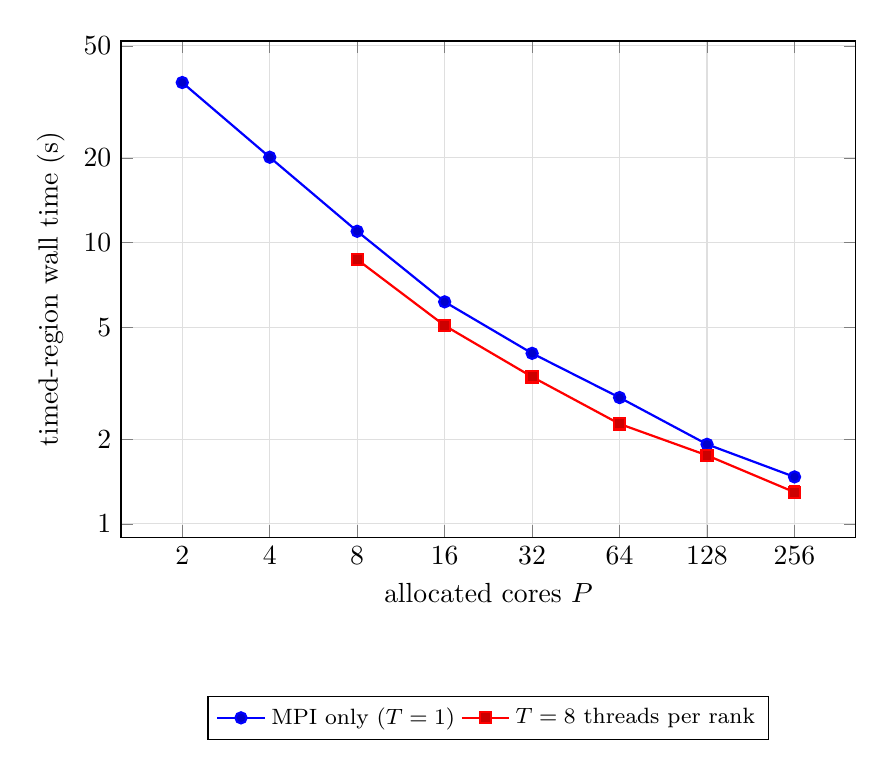
\begin{tikzpicture}
\begin{axis}[width=0.9\columnwidth, height=0.65\columnwidth, xlabel={allocated cores $P$}, ylabel={timed-region wall time (s)}, xmode=log, log basis x=2, log ticks with fixed point, ymode=log, ytick={1,2,5,10,20,50,100,200,500}, legend style={at={(0.5,-0.32)}, anchor=north, legend columns=2, font=\footnotesize}, legend cell align=left, grid=major, grid style={gray!25}]
\addplot+[mark=*, thick, error bars/.cd, y dir=both, y explicit] coordinates {(2,37.03) += (0,0.03858) -= (0,0.009955) (4,20.09) += (0,0.007634) -= (0,0.06447) (8,10.96) += (0,0.01349) -= (0,0.03468) (16,6.151) += (0,0.01692) -= (0,0.01315) (32,4.036) += (0,0.01958) -= (0,0.02826) (64,2.81) += (0,0.01345) -= (0,0.06373) (128,1.917) += (0,0.01298) -= (0,0.00859) (256,1.468) += (0,0.0133) -= (0,0.01316)};
\addlegendentry{MPI only ($T=1$)}
\addplot+[mark=square*, thick, error bars/.cd, y dir=both, y explicit] coordinates {(8,8.696) += (0,0.1684) -= (0,0.01753) (16,5.065) += (0,0.01414) -= (0,0.004754) (32,3.329) += (0,0.004293) -= (0,0.006183) (64,2.265) += (0,0.03151) -= (0,0.04496) (128,1.751) += (0,0.02158) -= (0,0.04165) (256,1.295) += (0,0.06983) -= (0,0.03696)};
\addlegendentry{$T=8$ threads per rank}
\end{axis}
\end{tikzpicture}
\caption{Strong-scaling runtime. $N=10^{6}$, median of repetitions; serial Barnes--Hut baseline on the same CPU model and build. Bars: fastest to slowest repetition. Vanda job 1535991: 64 of 72 cores on each of four Platinum 8452Y nodes (CN-047, CN-061, CN-064, CN-065), 3 interleaved repetitions.}
\label{fig:b4-strong-runtime}
\end{figure}
